\documentclass{article}

% Recommended, but optional, packages for figures and better typesetting:
\usepackage{microtype}
\usepackage{graphicx}
\usepackage{subfigure}
\usepackage{booktabs} % for professional tables
% \renewcommand{\baselinestretch}{1.2} 

\usepackage[colorlinks,
linkcolor=red,
anchorcolor=blue,
citecolor=blue
]{hyperref}

\usepackage{smile}

\usepackage{enumitem}
\usepackage{fullpage}




\title{IEMS-452 Matching Project Report}



\author{Zuyue Fu}
\begin{document}
\maketitle

\begin{abstract}
We solve matching problem in this project using combinatorial optimization method.   Our algorithm is  out-of-core, which ensures that  at any point of  the algorithm,  we do not process  more than 30\% of the edges in a graph.   Our code  is available  at \url{https://github.com/wuyuup/iems-452-proj.git}.  

\end{abstract}


\section{Introduction}

Max cardinality matching has a  long history, and  many existing algorithms  solve the  problem  exactly,  e.g.,  blossom algorithm.   Due to the increasing    sizes of graphs  considered in  recent  tasks,  algorithms that are out-of-core are  required.    In this course project,  we design  such an out-of-core algorithm,   which   will access at most 30\% of edges  at any  point  in the implementation of  our  algorithm.     


\section{Methodology}

Our method is  a heuristic-based augmenting path algorithm.  In specific,  our method consists of  two parts.   First,  we  implement a  greedy algorithm ,  where we  keep adding edges to the matching set until  no further  edges can be added.   Second,  repeatedly,  we   randomly  load 30\% edges  of  the graph  to find  augmenting paths  for the current matching set.   As the number of repetition  grows, such a  random  choice  of  30\% edges of the graph  ensures that   we  can finally   find   all   available   augmenting paths  with  a high probability.    We summarize the idea in Algorithm \ref{algo:1}. 

\begin{algorithm}
\caption{Heuristic-based Augmenting Path Algorithm}
\label{algo:1}
\begin{algorithmic}[1]
\STATE{{\bf Input:}  Graph $G = (V,E)$,  number of iteration \texttt{niter}    }
\STATE{{\bf Output:}  Matching $M$ }  
\STATE{ $M \gets \texttt{greedy}(G)$  }  \label{line:1}
\FOR{$n = 1, 2, \ldots, \texttt{niter}$}
\STATE{ Randomly select edge set $E'$ from $E$ such that $|E'| \leq 0.3 |E|$, let $G' \gets (V, E')$  }  \label{line:2}
\STATE{ $P \gets  \texttt{augmenting\_path}(G',M)$}  \label{line:3}
\STATE{ $M \gets M \Delta P$}
\ENDFOR
\end{algorithmic}
\end{algorithm}

In Line \ref{line:1} of Algorithm \ref{algo:1}, we  use  the greedy     algorithm \texttt{greedy} with $G$ as  the input.   Such a greedy     algorithm \texttt{greedy}  is easily  formalized  given previous  description; thus,  we omit  its details here.   Similarly, in Line \ref{line:3} of Algorithm \ref{algo:1},   we  use  the augmenting path  algorithm \texttt{augmenting\_path} with partial graph $G'$  and  current matching $M$ as  inputs.    

It is worthwhile to  remark that  the implementation of   Line \ref{line:2}   can be  in an out-of-core fashion.  In specific,  one may   randomly  read  30\% edges  in the graph   from the disk,  and only  save  these 30\%  edges in  the memory.  


\section{Numerical Experiment}\label{sec:num}

We   use graph data from  \url{https://northwestern.box.com/s/pz1at6ilfl323sxnkulbmsh6kde4z3fw}, which contains 21 graphs  with sizes of  optimal  matching vary from 0 to 10272.    Among these graphs,  the numbers of rows and columns of the  adjacency matrix  in   lp\_e226   do not matching.  To deal with this graph,  we  fill the adjacency  matrix  with zeros  to   match the dimension.  

To  obtain   the accuracy (i.e., optimality gap) of Algorithm \ref{algo:1},  we  use the package {NetworkX} \citep{hagberg2008exploring} to  obtain the size of the optimal  matching,  which is reported in Table \ref{tab:1}.    As required,  NetworkX  is only used to  obtain the optimal  matching, and is not used  for  any other purpose.  

We report the accuracy and standard deviations of  Algorithm \ref{algo:1}  with different choices  of \texttt{niter}.  

\begin{figure}[htbp] %  figure placement: here, top, bottom, or page
   \centering
   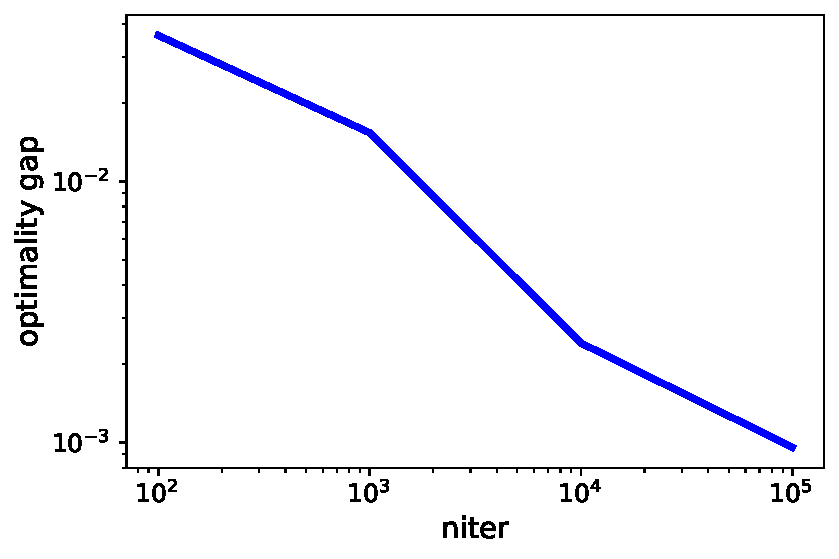
\includegraphics[width=3.2in]{1.pdf}
   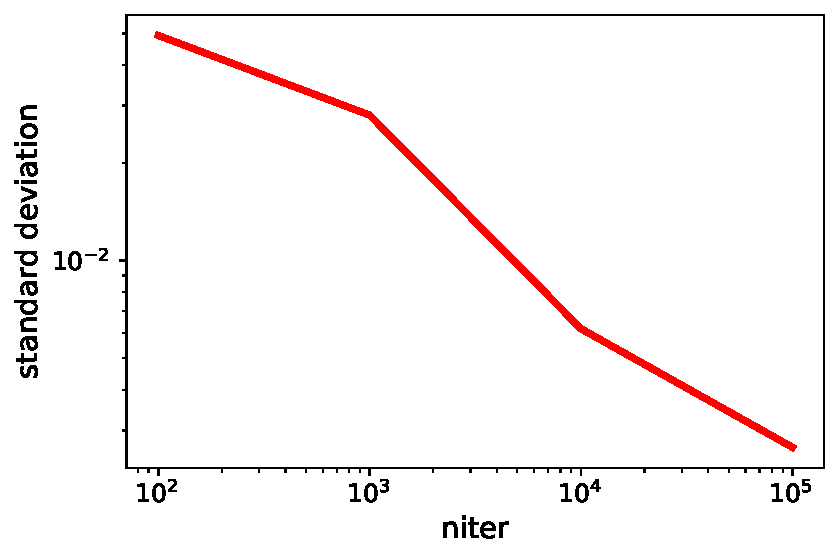
\includegraphics[width=3.2in]{2.pdf} 
   \caption{Optimality gaps and standard deviations of  Algorithm \ref{algo:1}  with  $\texttt{niter}\in \{10^2, 10^3, 10^4, 10^5\}$. }
   \label{fig:1}
\end{figure}

From Figure \ref{fig:1},  the choice $\texttt{niter}=10^5$ achieves the best  gap  0.096\% with standard deviation 0.00266.    For the completeness of  this report,   we report the accuracy  with $\texttt{niter}=10^5$ for each  graph in    Table \ref{tab:1}. 

% Requires the booktabs if the memoir class is not being used
\begin{table}[htbp]
   \centering
   %\topcaption{Table captions are better up top} % requires the topcapt package
   \begin{tabular}{|c|c|c|c|} % Column formatting, @{} suppresses leading/trailing space
   \hline
      graph    & opt. & ours & acc.  \\
      \hline
      sphere3      & 129 & 129 & 0 \\
               poli&792  &792 & 0 \\
               msc01440&720  &720 &0  \\
               mark3jac020sc& 4554 & 4551& 0.000659 \\
               lshp\_406&203  &203 &0  \\
               lp\_e226& 200 &200 &0  \\
               dwt\_72& 32 & 32& 0  \\
               dwt\_2680& 1340 &1339 &0.000746  \\
               dwt\_198&  99 & 99 & 0  \\
               can\_62 & 29 & 29 & 0  \\
               bcsstm26& 0   &  0 & 0 \\
               bcsstm02& 0 & 0& 0 \\
               bcsstm01& 0 & 0 & 0 \\
               bcsstk05& 76 & 76 & 0  \\
               bcspwr10 & 2576 & 2545 &  0.012\\
               bcspwr01 & 17  & 17 & 0 \\
               bayer04& 10272 & 10237 & 0.00341 \\
               b2\_ss& 544 &544 & 0 \\
               G17 & 400 & 400 & 0  \\
               G15 & 400 & 400& 0 \\
               662\_bus&  306 &305 &  0.00327 \\
       \hline
   \end{tabular}
   \caption{ Accuracy for each graph with $\texttt{niter}=10^5$.  }
   \label{tab:1}
\end{table}






\section{Concluding Remarks}
Such a method in Algorithm \ref{algo:1} does not guarantee that  we  will find  the optimal matching even when \texttt{niter} goes to infinity, since  we do not deal with possible blossoms in the graph.   However,  such a  method does achieve great  results  on the given set of graphs,  as  we show in \S\ref{sec:num}. 


\bibliographystyle{ims}
\bibliography{ref}


\end{document}


